 \documentclass[
	a4paper
]{scrreprt}

%%% PACKAGES %%%

% add unicode support and use german as language (change to have different auto generated titles like Management Summary)
\usepackage[utf8]{inputenc}
% \usepackage[ngerman]{babel}

% Use Helvetica as font
\usepackage[scaled]{helvet}
\renewcommand\familydefault{\sfdefault}
\usepackage[T1]{fontenc}

\usepackage{float}

% Better tables
\usepackage{tabularx}

% Better enumerisation env
\usepackage{enumitem}

% Use graphics
\usepackage{graphicx}

% Have subfigures and captions
\usepackage{subcaption}

% Be able to include PDFs in the file
\usepackage{pdfpages}

% Have custom abstract heading
\usepackage{abstract}

% Need a list of equation
\usepackage{tocloft}
\usepackage{ragged2e}

% Better equation environment
\usepackage{amsmath}

% Symbols for most SI units
\usepackage{siunitx}

\usepackage{csquotes}

% Change page rotation
\usepackage{pdflscape}

% Symbols like checkmark
\usepackage{amssymb}
\usepackage{pifont}

\usepackage[absolute]{textpos}

% Code listing package
\usepackage{listings}
\usepackage{color}

\definecolor{dkgreen}{rgb}{0,0.6,0}
\definecolor{gray}{rgb}{0.5,0.5,0.5}
\definecolor{mauve}{rgb}{0.58,0,0.82}

\lstset{frame=tb,
  language=Python,
  aboveskip=3mm,
  belowskip=3mm,
  showstringspaces=false,
  columns=flexible,
  basicstyle={\small\ttfamily},
  numbers=none,
  numberstyle=\tiny\color{gray},
  keywordstyle=\color{blue},
  commentstyle=\color{dkgreen},
  stringstyle=\color{mauve},
  breaklines=true,
  breakatwhitespace=true,
  tabsize=3
}


% Glossary, hyperref, babel, polyglossia, inputenc, fontenc must be loaded before this package if they are used
% \usepackage{glossaries}
\usepackage[automake]{glossaries}
% Redefine the quote charachter as we are using ngerman
\GlsSetQuote{+}
% Define the usage of an acronym, Abbreviation (Abbr.), next usage: The Abbr. of ...
\setacronymstyle{long-short}

% Bibliography & citing
\usepackage[
	backend=biber,
	style=apa,
	bibstyle=apa,
	citestyle=apa,
	sortlocale=en_EN
	]{biblatex}
\addbibresource{bibliography.bib}
% \DeclareLanguageMapping{ngerman}{ngerman-apa}

% Clickable Links to Websites and chapters
% From the documentation: "Make sure it comeslastof your loaded packages, to give it a fighting chance of not beingover-written, since its job is to redefine many LATEX commands"
\usepackage{hyperref}

%%% COMMAND REBINDINGS %%%
\newcommand{\tabitem}{~~\llap{\textbullet}~~}
\newcommand{\xmark}{\ding{55}}
\newcommand{\notmark}{\textbf{\textasciitilde}}

% Define list of equations - Thanks to Charles Clayton: https://tex.stackexchange.com/a/354096
\newcommand{\listequationsname}{\huge{Table of Equations}}
\newlistof{myequations}{equ}{\listequationsname}
\newcommand{\myequations}[1]{
	\addcontentsline{equ}{myequations}{\protect\numberline{\theequation}#1}
}
\setlength{\cftmyequationsnumwidth}{2.3em}
\setlength{\cftmyequationsindent}{1.5em}

% Usage {equation}{caption}{label}
% \indexequation{b = \frac{\pi}{\SI{180}{\degree}}\cdot\beta\cdot 6378.137}{Bogenlänge $b$ des Winkels $\beta$ mit Radius 6378.137m (Distanz zum Erdmittelpunkt am Äquator)}{Bogenlaenge}
\newcommand{\indexequation}[3]{
	\begin{align} \label{#3} \ensuremath{\boxed{#1}} \end{align}
	\myequations{#3} \centering \small \textit{#2} \normalsize \justify }

% Nested Enumeratelist credit to https://tex.stackexchange.com/a/54676
\newlist{legal}{enumerate}{10}
\setlist[legal]{label*=\arabic*.}

%%% PATH DEFINITIONS %%%
% Define the path were images are found
\graphicspath{{./img/}{./appendix/}}

%%% GLOSSARY ENTRIES %%%
\makeglossaries
\newglossaryentry{rouge}{
  type=\acronymtype,
  name={ROUGE},
  description={Recall-Oriented Understudy for Gisting Evaluation},
  first={ROUGE}
}
\newglossaryentry{mcrmse}{
  type=\acronymtype,
  name={MCRMSE},
  description={Mean Columnwise Root Mean Squared Error},
  first={Mean Columnwise Root Mean Squared Error (MCRMSE)}
}
\newglossaryentry{rmse}{
  type=\acronymtype,
  name={RMSE},
  description={Root Mean Squared Error},
  first={Root Mean Squared Error (RMSE)}
}
\newglossaryentry{mse}{
  type=\acronymtype,
  name={MSE},
  description={Mean Squared Error},
  first={Mean Squared Error (MSE)}
}
\newglossaryentry{mae}{
  type=\acronymtype,
  name={MAE},
  description={Mean Absolute Error},
  first={Mean Absolute Error (MAE)}
}
\newglossaryentry{n-gram}{
    name={n-gram},
    plural={n-grams},
    description={A contiguous sequence of n items (words, characters, etc.) in a text},
}
\newglossaryentry{skip-gram}{
    name={skip-gram},
    plural={skip-grams},
    description={An n-gram model where not all consecutive items in a sequence are included, but instead, some elements are skipped},
}

\newglossaryentry{skip-bigram}{
    name={skip-bigram},
    description={A pair of items in a sequence where some elements are skipped}
}
\newglossaryentry{lcs}{
	name={LCS},
	description={Longest Common Subsequence},
	first={Longest Common Subsequence (LCS)},
}
\newglossaryentry{token}{
	name={token},
	description={Individual units, such as words or subwords, extracted from a given text or sequence}
}
\newglossaryentry{bleu}{
	name={BLEU},
	description={Bilingual Evaluation Understudy}
}
\newglossaryentry{meteor}{
	name={METEOR},
	description={Metric for Evaluation of Translation with Explicit Ordering}
}
\newglossaryentry{perplexity}{
	name={Perplexity},
	description={A quantitative measure that assesses how well a language model predicts a given set of text}
}

\newglossaryentry{goss}{
	name={GOSS},
	description={Gradient-based One Side Sampling}
}
\newglossaryentry{efb}{
	name={EFB},
	description={Exclusive Feature Bundling}
}
\newglossaryentry{gbdt}{
	name={GBDT},
	description={Gradient-Boosted Decision Trees
}
}
\newglossaryentry{nn}{
	name={NN},
	description={Neural Network},
}
\newglossaryentry{rnn}{
	name={RNN},
	description={Recurrent Neural Network},
}
\newglossaryentry{lstm}{
	name={LSTM},
	description={Long Short-Term Memory},
}
\newglossaryentry{wandb}{
	name={WandB},
	description={Weights \& Biases},
	first={Weights \& Biases (WandB)},
}
\newglossaryentry{w2v}{
	name={Word2Vec},
	description={A technique for obtaining vector representations of words},
}

\newglossaryentry{stemming}{
	name={stemming},
	description={Reducing a word to its word stem},
}
\newglossaryentry{lemmatization}{
	name={lemmatization},
	description={Breaking down a word to its root meaning},
}
\newglossaryentry{hidden-layer}{
	name={hidden layer},
	description={The layer(s) of neurons that are between the input and output layers},
}
\newglossaryentry{hidden-dim}{
	name={hidden-dim},
	description={The number of neurons in a hidden layer},
}
\newglossaryentry{activation function}{
	name={activation function},
	description={A non-inear function which calculates the output of a neuron},
}

\newglossaryentry{max_length}{
	name={Max length},
	description={Upper limit on the number of tokens of sequence},
}
\newglossaryentry{batch_size}{
	name={Batch size},
	description={Specifies the number of data samples processed simultaneously in one iteration},
}
\newglossaryentry{epoch}{
	name={Epoch},
	description={Denotes the number of times the entire training dataset is passed through the model},
}
\newglossaryentry{lr}{
	name={Learning rate},
	description={Controls the size of the steps taken during the optimization process},
}
\newglossaryentry{weight_decay}{
	name={Weight decay},
	description={Regularization technique that applies a penalty to the magnitude of the model's weights},
}

\newglossaryentry{lgbm_numofest}{
	name={Number of Estimators},
	description={Controls the number of decision trees in the model},
}
\newglossaryentry{lgbm_lr}{
	name={Learning Rate},
	description={Controls the learning speed},
}
\newglossaryentry{lgbm_colsamp}{
	name={Colsample Bytree},
	description={Fracture of features used to train model (0.75 for example means that 75\% of the features are used for training)},
}
\newglossaryentry{lgbm_regalp}{
	name={Reg Alpha},
	description={Used to penalize features},
}


%%% DOCUMENT %%%

\begin{document}

version https://git-lfs.github.com/spec/v1
oid sha256:bf3cefcf1c21c22f0466ec74964ef38b5d1b61c6a2d4353983a3ea4bbd192b66
size 583


\pagenumbering{Roman}

\chapter*{Eidesstattliche Erklärung}

Wir erklären hiermit, dass wir die vorliegende Arbeit selbständig und ohne unerlaubte fremde Hilfe angefertigt haben, alle verwendeten Quellen, Literatur und andere Hilfsmittel angegeben haben, wörtlich oder inhaltlich entnommene Stellen als solche kenntlich gemacht haben, das Vertraulichkeitsinteresse des Auftraggebers wahren und die Urheberrechtsbestimmungen der Hochschule Luzern respektieren werden.


\vspace{50mm}
\begin{tabular}{@{}p{2.5in}@{}}
\hrulefill \\
Jonathan Carona \\
Hochschule Luzern
\end{tabular}

\vspace{25mm}
\begin{tabular}{@{}p{2.5in}@{}}
\hrulefill \\
Josef Rittiner \\
Hochschule Luzern
\end{tabular}

\vspace{25mm}
\begin{tabular}{@{}p{2.5in}@{}}
\hrulefill \\
Tharrmeehan Krishnathasan \\
Hochschule Luzern
\end{tabular}

\begin{abstract}
\noindent
This project revolved around the Kaggle Challenge: CommonLit - Evaluate Student Summaries. The aim of this challenge was to create a machine learning model, which could accurately assess the quality of summaries written by students in grades 3-12. Using the data provided by the challenge, which contained the summaries of over 7'000 students across four different topics, the team developed three distinct models.\\
The ROUGE-Based Model is a Neural Network, which uses ROUGE metrics as it’s input features. The LightGBM Model uses an array of scores, which can determine readability, complexity and the grade level of a summary. The DeBerta Transformer, a state-of-the-art language model which balances out the two while also considering the specific task the students were asked to capture in their summary.\\
These three models collectively form the final Ensemble Model. Each model independently preprocesses the texts and generates predictions. The Ensemble Model weighs the contributions of each model to produce a final score. The results showcase respectable performance in the Kaggle competition, placing 975th out of a total 2'065 participants.
\end{abstract}

\tableofcontents

\clearpage
\pagenumbering{arabic}

\chapter{Introduction}
\label{ch:introduction}

\section{Problem Statement}
This project stems from the Kaggle Challenge: Evaluate Student Summaries,\footnote{\href{https://www.kaggle.com/competitions/commonlit-evaluate-student-summaries}{CommonLit - Evaluate Student Summaries - Website}} which was hosted by CommonLit. The objective of this competition was to assess the quality of summaries written by students in grades 3-12.\\
This involved developing a machine learning model to predict the scores given by human annotators for two different metrics: "Content" and "Wording", as described in \hyperref[fig:content-and-wording]{Figure~\ref{fig:content-and-wording}}.\\
\begin{figure}[h]
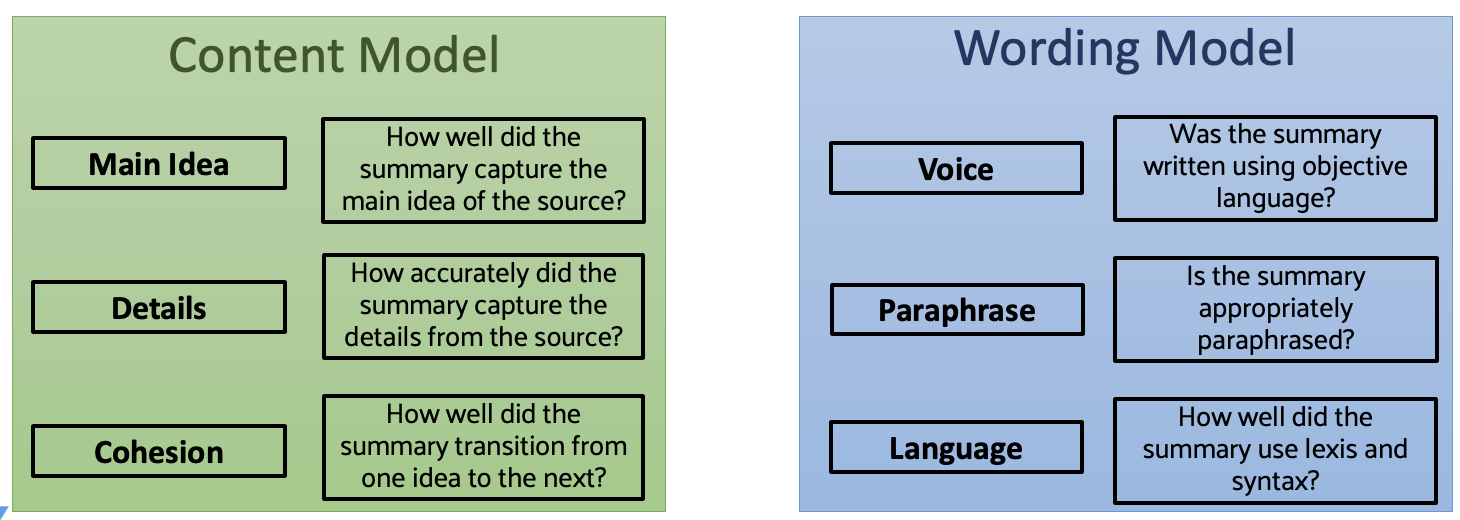
\includegraphics[keepaspectratio, width=\textwidth]{img/content_wording.png}
\caption[Description of Content and Wording]{Source: \href{https://www.kaggle.com/competitions/commonlit-evaluate-student-summaries/discussion/424402\#2349973}{CommonLit - Evaluate Student Summaries}}
\label{fig:content-and-wording}
\end{figure}\\
The human annotators were instructed to ignore grammar and spelling when evaluating the summaries. Additionally, the annotators were unaware of the students' grade levels. Meaning all summaries, regardless of what grades the students were in, were evaluated equally. This is also reflected in the data. There is no information on the students, only a unique student ID and the summary itself, together with its wording and content scores and an ID to identify to which reference text it was based on. Further details about the data are provided in \hyperref[ch:data]{Chapter~\ref{ch:data}}.

\pagebreak
\subsection{Background and Motivation of Problem}
CommonLit is a nonprofit organization dedicated to promoting reading, writing, communication, and problem-solving skills in students. Writing summaries is a crucial skill that encompasses reading comprehension, writing proficiency, and critical thinking. Unfortunately, it is a time-consuming task for teachers to read, correct, and grade students’ summaries, limiting the opportunities for students to practice these skills.\\
Being able to automatically evaluating students' writing would significantly reduce the workload for teachers. But there is a scarcity of datasets containing student writing. As a result, current techniques for summary evaluation primarily focus on automatically generated summaries rather than those created by humans, let alone students.

\section{Goal of this Work}
The primary objective of this project was to leverage the data provided by the challenge and develop a model capable of automatically predicting accurate scores. The Kaggle challenge presented two distinct prize categories: Leaderboard and Efficiency. Our focus was on the Leaderboard category, as the we believed that prioritizing accuracy over efficiency would provide a more valuable learning experience. Moreover, deliberately overfitting models was avoided, as we deemed it 
%inconsistent with the spirit of the challenge and
unrepresentative of real-world projects.

\section{Evaluation Function}
Submissions to the challenge were scored using the \gls{mcrmse}, calculated as follows:

\begin{equation}\label{eq:mcrmse}
    MCRMSE = \frac{1}{N_t} \sum_{j=1}^{N_t} \sqrt{\frac{1}{n} \sum_{i=1}^{n} (y_{ij} - \hat{y}_{ij})^2}
\end{equation}
\myequations{Mean Columnwise Root Mean Squared Error}

\noindent $N_t$ represents the number of target columns, with $N_t = 2$ in this case (one column for the content scores and one for the wording scores). The variable $n$ corresponds to the number of rows, i.e. the total number of summaries to be evaluated. And the variables $y$ and $\hat{y}$ denote the actual and predicted values, respectively.\\
In short, the \gls{mcrmse} is obtained by computing the \gls{rmse} for each of the two metrics: content and wording. The final score is then determined by averaging all the calculated \glspl{rmse} across those two metrics.\\
The range of the \gls{mcrmse} is non-negative, with 0 being the theoretical best possible score. (It can be calculated easily in Python
%\footnote{\href{https://www.python.org/}{Python - Website}}
using the scikit-learn
%\footnote{\href{https://scikit-learn.org/}{scikit-learn - Website}}
library.)
\begin{lstlisting}[language=Python]
from sklearn.metrics import mean_squared_error
rmse_content = mean_squared_error(y_true[0], y_pred[0], squared=False)
rmse_wording = mean_squared_error(y_true[1], y_pred[1], squared=False)
mcrmse = 1/2 * (rmse_content + rmse_wording)
\end{lstlisting}

% Josef

version https://git-lfs.github.com/spec/v1
oid sha256:8fec1fdd4176ff5f6ca7bd3af44be61fa9704ffe8d3429780df92bf5a9110696
size 55

% State of the Art and Machine Learning Theory - All

version https://git-lfs.github.com/spec/v1
oid sha256:6a882c9d0cae23b9bb392d25da3a703e29fb07148742ea28d44f9ed16eb50ab6
size 99

% Data Quality Assesment - Tarrmeehan

\chapter{Modeling}
% Ergebnisse über die einzelnen Iterationen
% Preprocessing
% Architecture
% Hyperparameter tuning
% Training
% Limitations
% What didn't work (separate subsection)
% --> Model Evaluation


\section{Models}

\subsection{ROUGE-Based Model}
The ROUGE-Based Model is a simple \glsdisp{nn}{Neural Network} utilizing \gls{rouge} scores as its inputs. It was designed to predict the content score based on the summary and the reference text. While it does also predict the wording score, it does not perform as well on it.\\
The inspiration for this model arose during the exploration of existing methods for text evaluation. Among other metrics, such as \gls{bleu}, \gls{meteor} and \gls{perplexity}, \gls{rouge} stood out, as it was originally designed for assessing summaries.
However, as quoted in
\hyperref[sec:rouge_theory]{Chapter \ref{sec:rouge_theory}},
the \gls{rouge} Measures compare a computer-generated summary to a human-written one. So, for this project, it was adapted by substituting the machine-written summary with that of a student and replacing the (ideal) human-written summary with the full reference text.\\
\subsubsection{Model Architecture}
The ROUGE-Based Model consists of two distinct steps: the calculation of \gls{rouge}-scores and the forward pass through the neural network, as illustrated in
\hyperref[fig:rouge-based-model]{Figure~\ref{fig:rouge-based-model}}.
The \gls{rouge}-scores are computed from the \glsdisp{token}{tokenized} reference text and summary, after their stopwords were removed. The Precision, Recall, and F1-Score from the ROUGE-scores, along with the normalized length of the summary, serve as inputs to the network. The network then outputs the predicted content and wording scores for the summary.
\begin{figure}[H]
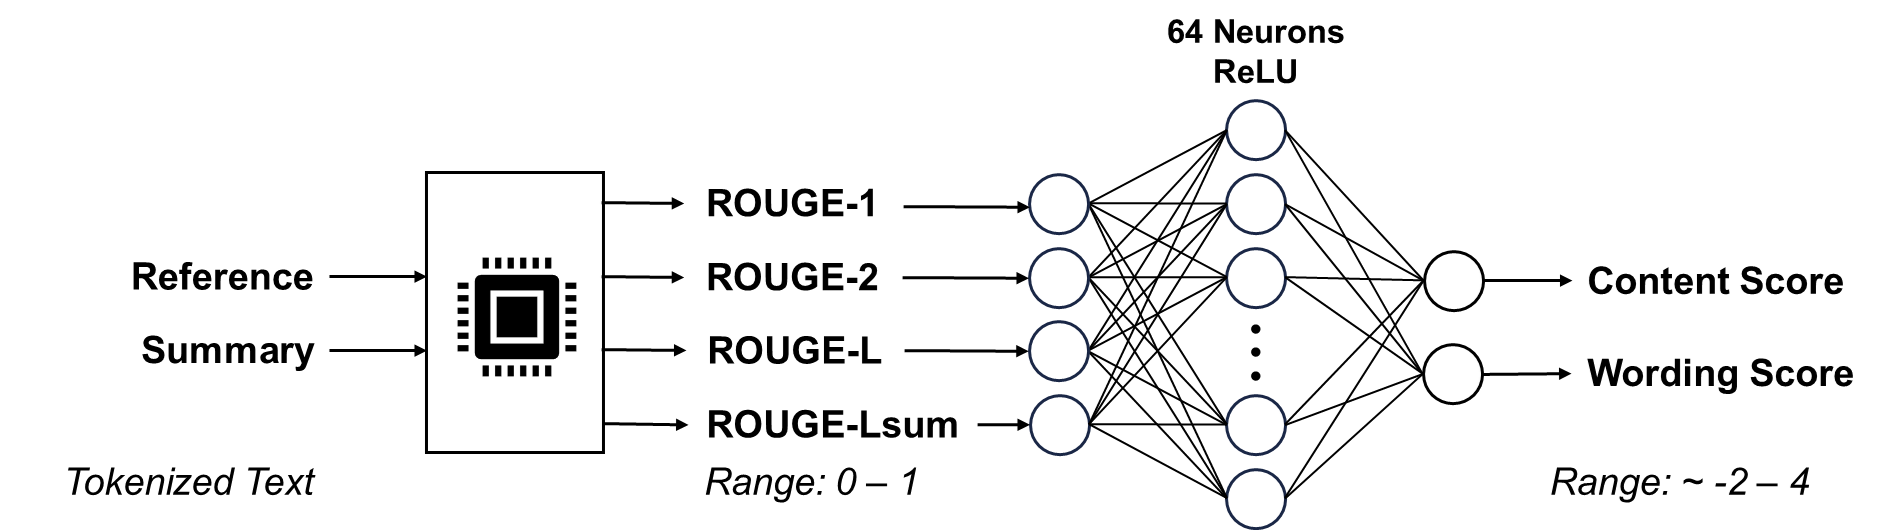
\includegraphics[keepaspectratio, width=\textwidth]{ROUGE-Based-Model.png}
\caption[ROUGE-Based Model Architecture]{Architecture of the ROUGE-Based Model.}
\label{fig:rouge-based-model}
\end{figure}

% \subsubsection{Hyperparameters}
% 
% \begin{itemize}
%     \item \textbf{Stopword Removal:} Determines whether stopwords are removed during processing.
%     \item \textbf{Stemming:} Controls whether stemming is applied to reduce words to their root form.
%     \item \textbf{Lemmatization:} Controls whether lemmatization is used to obtain the base form of words.
%     \item \textbf{ROUGE metrics:} Specifies what combination ROUGE metrics are used..
%     \item \textbf{Hidden-dim:} Sets the number of hidden layers in the neural network.
%     \item \textbf{Hidden-layers:} Determines the number of hidden layers in the neural network.
%     \item \textbf{Activation function:} Specifies the activation function applied in the neural network.
%     \item \textbf{Learning rate:} Learning Rate.
%     \item \textbf{Epochs:} Determines the number of times the entire training dataset is passed through the neural network.
% \end{itemize}

\subsubsection{Hyperparameter Tuning}

During the development and training of the ROUGE-Based Model, various hyperparameters were explored and tuned using the Optuna\footnote{\href{https://optuna.org/}{Optuna - Website}} library. It was found, that removing stopwords and applying \gls{stemming} or \gls{lemmatization} had little to no impact on the models performance. Therefore stopwords were removed to reduce the number of \glspl{token} when calculating the \gls{rouge} scores and neither stemming nor lemmatization were applied, as they were unnecessary. For the models inputs, specific \gls{rouge} scores were used, including ROUGE-1, ROUGE-2, ROUGE-L, and ROUGE-Lsum. These scores were calculated using the Python library 'rouge-score'.\footnote{\href{https://pypi.org/project/rouge-score/}{rouge-score library - PyPI Website}}
It's worth noting that later in the project, another library called 'rouge-metric'\footnote{\href{https://pypi.org/project/rouge-metric/}{rouge-metric library - PyPI Website}}
was found, which could calculate the additional gls{rouge} scores. However, considering the likely marginal gains and to maintain consistency, it was decided not to re-implement the model with the new library.\\
Given the nature of this model and the task, where the network primarily maps the \gls{rouge} scores (ranging from 0 to 1) into the content and wording scores (ranging from -2 to 4), the \gls{nn} was quite robust against overfitting. Changes in the number of hidden neurons and \glspl{hidden-layer} (as log as there was at least one \gls{hidden-layer}) had minimal impact on performance. Notably, the selection of the \gls{activation function} played a bigger role; logistic functions like Sigmoid and tanh demonstrated poorer performance. However, ReLU and Leaky ReLU showed better results, ultimately leading to the adoption of ReLU in the final model.

\begin{itemize}
    \item \textbf{Stopword Removal:} Stopwords were removed.
    \item \textbf{\glsdisp{stemming}{Stemming} \& \glsdisp{lemmatization}{Lemmatization}:} Neither \gls{stemming} nor \gls{lemmatization} was used.
    \item \textbf{ROUGE Metrics:} \gls{rouge}-1, \gls{rouge}-2, \gls{rouge}-L, \gls{rouge}-Lsum
    \item \textbf{\glsdisp{hidden-layer}{Hidden-Layers}:} 1 Hidden Layer
    \item \textbf{\glsdisp{hidden-dim}{Hidden-Dim}:} 64 Neurons
    \item \textbf{\glsdisp{activation function}{Activation Function}:} ReLU
    \item \textbf{\glsdisp{lr}{Learning Rate}:} 0.01
    \item \textbf{\glsdisp{epoch}{Epochs}:} 10
\end{itemize}
%\begin{figure}[H]
%
\includegraphics[keepaspectratio]{placeholder.png}
%\caption{\textbf{\textit{Hyperparameter Importance Plot(s) - Placeholder Text}}}
%\label{fig:rouge-hyperparameter-importance}
%\end{figure}

\subsubsection{Training}
The models \gls{nn} is initialized with random weights. Before training, it is also given the mean length (number of characters) and the standard deviation in length of the summaries in the training set. These two additional values are used to normalize the lengths of summaries, when passing them to the network. Since there is no upper bound for how long a summary can be, Z-Score Normalization was applied: %$z=\frac{x-\mu}{\sigma}$
\begin{equation}\label{eq:z-score}
    z=\frac{x-\mu}{\sigma}
\end{equation}
\myequations{Z-Score Normalization}
Where $z$ is the normalized length $x$ of a summary. $\mu$ is the mean length of the summaries in the trainings set and $\sigma$ the standard deviation.\\
Since the \gls{rouge} metrics have no learnable parameters, the python library 'rouge-score' can be used to precalculate these scores prior to training.
These precalculated scores are used as inputs to train the network, using the \gls{mse} loss function over 10 training \glspl{epoch}.

\subsubsection{Limitations}
It's important to note that this model only receives the summary and the reference text the summary was based on. It does not consider the specific task asked of the students. In cases where the prompt asks for specifics on one part of the text, a summary focusing on that prompt may be evaluated as worse than a summary that stays more general.\\
The model also doesn't know what words were used, only whether they overlap with the reference. Therefore, it cannot determine whether objective and neutral language was used or how well lexis and syntax was used. Due to these limitations it was expected, that this model performs better on the content score, and poorly on the wording score. (Also as evident by the correlation matrix; \hyperref[fig:rouge-correlation-matrix]{Figure~\ref{fig:rouge-correlation-matrix}}.)

\begin{figure}[h]
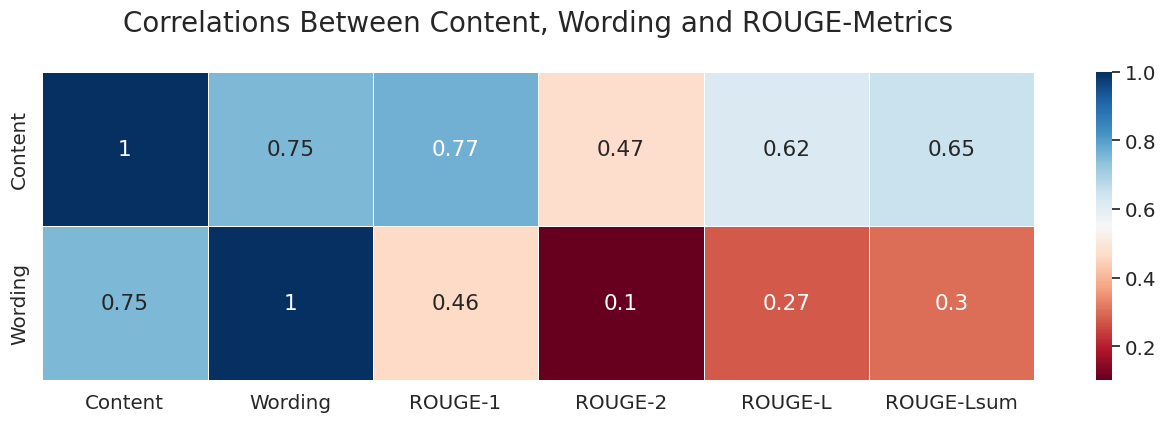
\includegraphics[keepaspectratio, width=\textwidth]{rouge_correlation_matrix.png}
\caption[ROUGE Metrics Correlation Matrix]{Correlations between Content and Wording scores and the used ROUGE Metrics}
\label{fig:rouge-correlation-matrix}
\end{figure}

\pagebreak
\subsection{Transformer}
%This section delves into how the transformer was implemented and tuned for the given task.
\subsubsection{Motivation}
In the past few years, transformers have risen in popularity in the NLP space. 
Student summaries have mostly long sequence lengths and require an efficient and capable architecture to fit the data.
Transformers are a perfect fit for the challenge at hand.

\subsubsection{Transformer selection}
When choosing the most fitting and optimal transformer multiple factors must be taken into consideration.
This would be the type of transformer for instance or how the attention mechanism was implemented.
Nevertheless, from just observing the desired result, which is predicting two continuous values, several factors can already be decided on.
Encoder-only models were chosen because there is no need for decoders, as there is nothing to decode.
From that observation, the team searched for suitable models on HuggingFace\footnote{\href{https://huggingface.co/}{HuggingFace - Website}}, a platform listing various transformer implementations. The search focused on encoder-only models, sorted by popularity.
Additionally, the complexity of the transformers was considered, along with trials of both uncased and cased models to assess their impact on performance.
All tested implementations were variations of BERT, primarily due to the team's limited familiarity and expertise with non-BERT-based models.\\

\noindent The best performing implementation was found as follows:
Since the public data only consists of four possible topics and the private data set of an unknown number of topics, a great importance on generalization was set.
Due to this, the cross-validation technique Group-K Fold was used. With this method the generalization performance can be estimated on unseen topics.
The models are trained on the training set using the HuggingFace Transformers library and the \gls{rmse} of the content and wording score, and the combination of \gls{mcrmse} were used to compute the metrics:

\vspace{1em}

\begin{lstlisting}
def compute_mcrmse(eval_pred):
    preds, labels = eval_pred

    col_rmse = np.sqrt(np.mean((preds - labels) ** 2, axis=0))
    mcrmse = np.mean(col_rmse)

    return {
        "content_rmse": col_rmse[0],
        "wording_rmse": col_rmse[1],
        "mcrmse": mcrmse,
    }
\end{lstlisting}

\vspace{2em}

\noindent When running the test all models had the exact same hyperparameter configuration:%. The following hyperparameters were used:
\begin{itemize}
	\item \textbf{Input:} The tokenized padded or truncated student-written summary.
	\item \textbf{\gls{max_length}:} 512. This was chosen since most of the BERT models have 512 as maximum length.
	\item \textbf{\gls{batch_size}:} 8
    \item \textbf{\glspl{epoch}:} 8
    \item \textbf{\gls{lr}:} 0.0001
    \item \textbf{\gls{weight_decay}:} 0.01
\end{itemize}
\textbf{NOTE:} Hyperparameters which are not listed above use the default settings from the HuggingFace Library.

\begin{figure}[H]
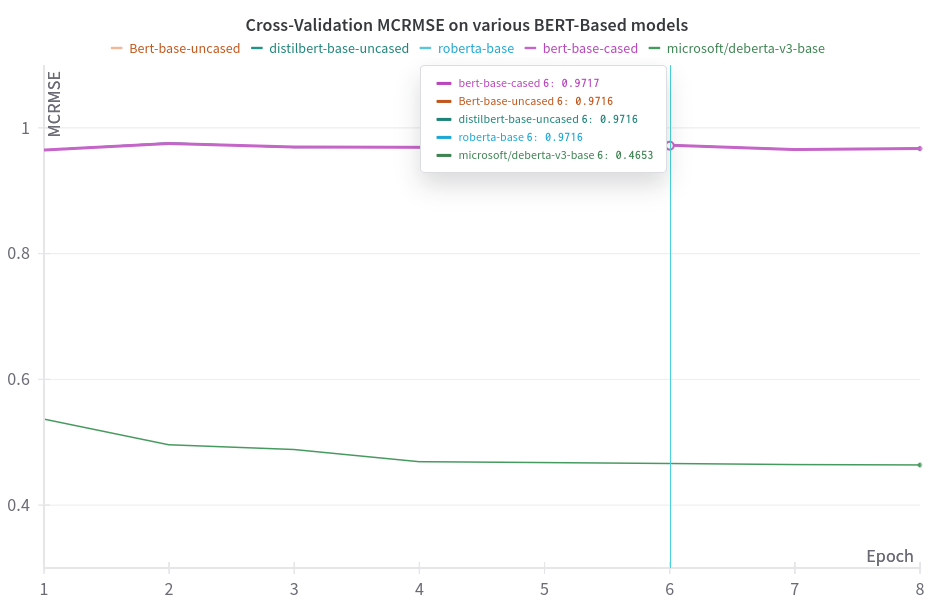
\includegraphics[keepaspectratio, width=\textwidth]{img/cross-validation-performance.png}
\caption{Cross-Validation MCRMSE Score Evolution on various BERT-Based models}
\label{fig:cross-validation}
\end{figure}
\vspace{1em}

The above visualization distinctly highlights a standout performer. All BERT-based models, except for DeBERTa fail to generalize effectively.
It is noteworthy that the performance metrics of models other than DeBERTa are quite similar, suggesting minimal variance among them. Additionally, the comparison of uncased and cased BERT-based models indicates that the casing does not significantly influence performance outcomes.
A possible reason for DeBERTa outperforming, and also what it makes it different compared to the other BERT-Based models, is the disentangled attention mechanism.

\subsubsection{Prompt Engineering}
When using transformers, using an optimized prompt has been proven to achieve better results.
Various experiments using different combinations of features from the data were conducted.
A logical combination of the features would be to use the student-written text together with the prompt text.
After further experimenting, adding the prompt question and using a natural language style prompt improved performance.

\begin{figure}[H]
\begin{center}
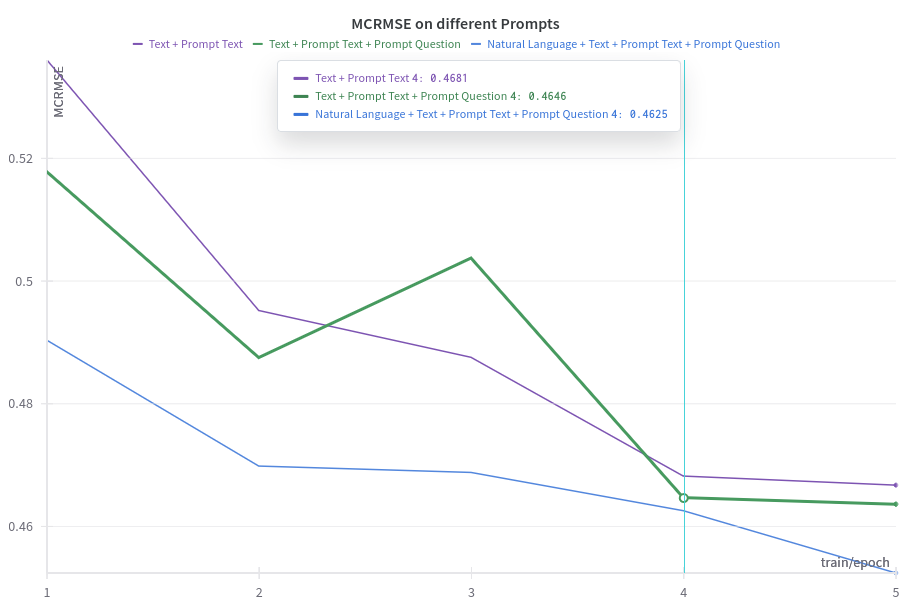
\includegraphics[keepaspectratio, width=\textwidth]{img/prompts.png}
\caption{MCRMSE Score Evolution on different Prompts}
\label{fig:prompts}
\end{center}
\end{figure}

\vspace{1em}

By using a natural language style prompt, verbs and objectives were used to specify the goal of the problem at hand.
The final prompt the transformer uses is the following:

\begin{quote}
    ``Evaluate the content and wording score of this summary: [SEP] \textbf{text} [SEP] The summary must answer the following prompt: [SEP] \textbf{prompt question} [SEP] The prompt is related towards the following original text: [SEP] \textbf{prompt text}''
\end{quote}

\subsubsection{Model Architecture}
The model uses three features from the dataset which are the student-written summary, the prompt text, and the prompt question.
These get formatted into the aforementioned prompt and \glsdisp{token}{tokenized}. The tokenizer pads or truncates the prompt to the max length.
The network then outputs the content and wording scores for the summary.

\begin{figure}[H]
\begin{center}
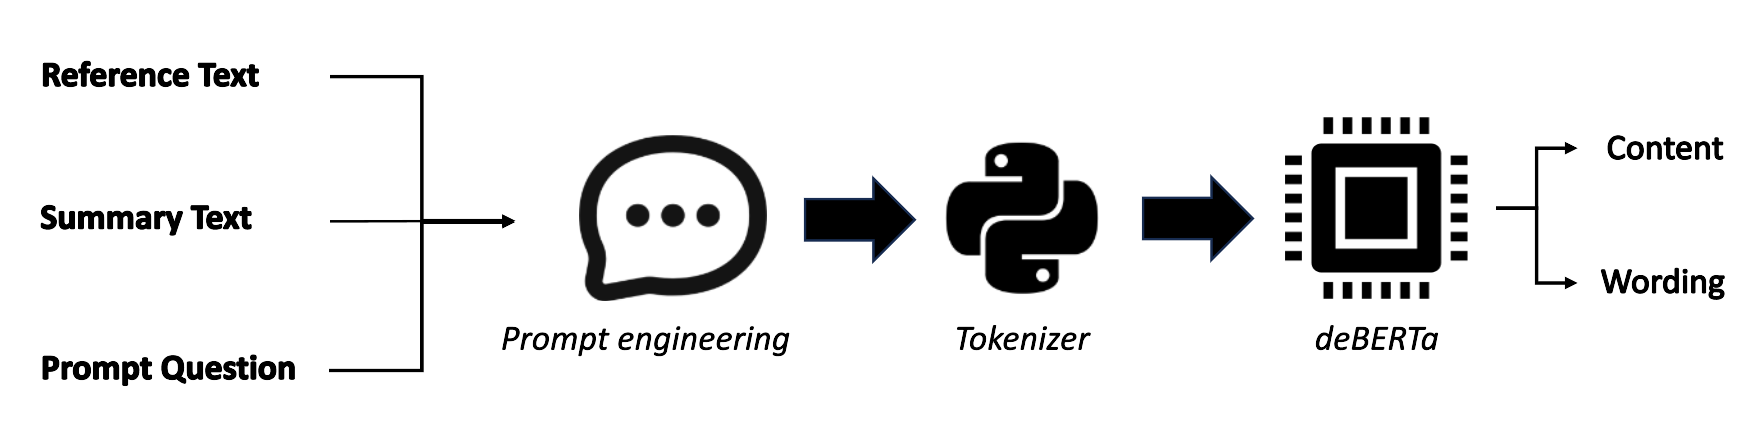
\includegraphics[keepaspectratio, width=0.8\textwidth]{img/transformer_architecture.png}
\caption{Transformer Pipeline}
\label{fig:transformer_architecture}
\end{center}
\end{figure}
\subsubsection{Hyperparameter tuning}
\subsubsection*{Layer fine-tuning}
DeBERTa contains twelve encoding layers. The Transformer model was downstreamed by freezing the bottom N layers.
After iterating and freezing each layer, the best performing iteration was freezing at layer 9:

\begin{figure}[H]
\begin{center}
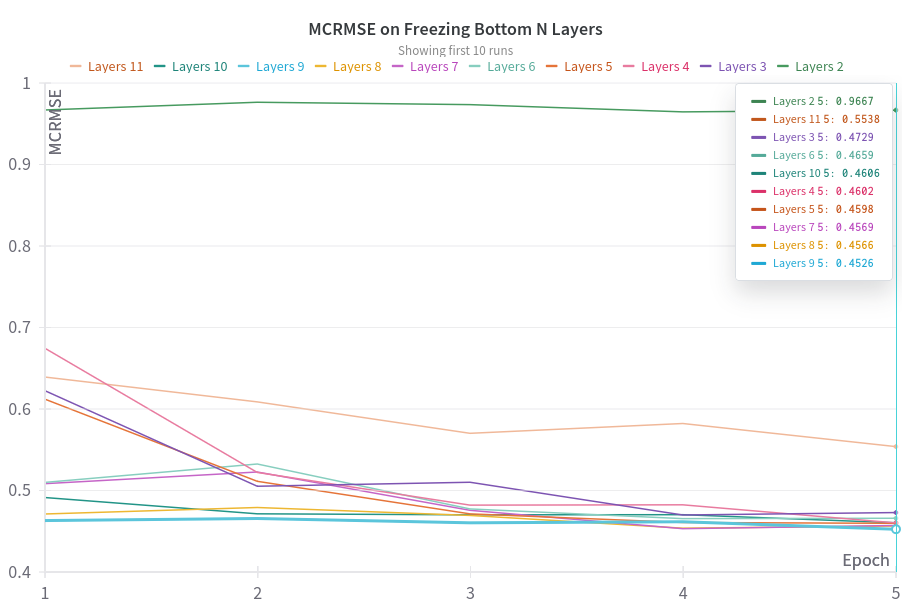
\includegraphics[keepaspectratio, width=0.86\textwidth]{img/n_layers.png}
\caption{MCRMSE Score Evolution on freezing N Layers}
\label{fig:n_layers}
\end{center}
\end{figure}
\subsubsection*{Max length fine-tuning}
Configuring the max length was essential, because if the max length is too short it could cut out important information of the prompt.
A logical conclusion would be that a higher max length would lead to better performance. However, sequence lengths over 1024 led to worse performance.
It is speculated that the text of the prompt exceeding 1024 \glspl{token} may become overly detailed, potentially impacting the results negatively.

\begin{figure}[H]
\begin{center}
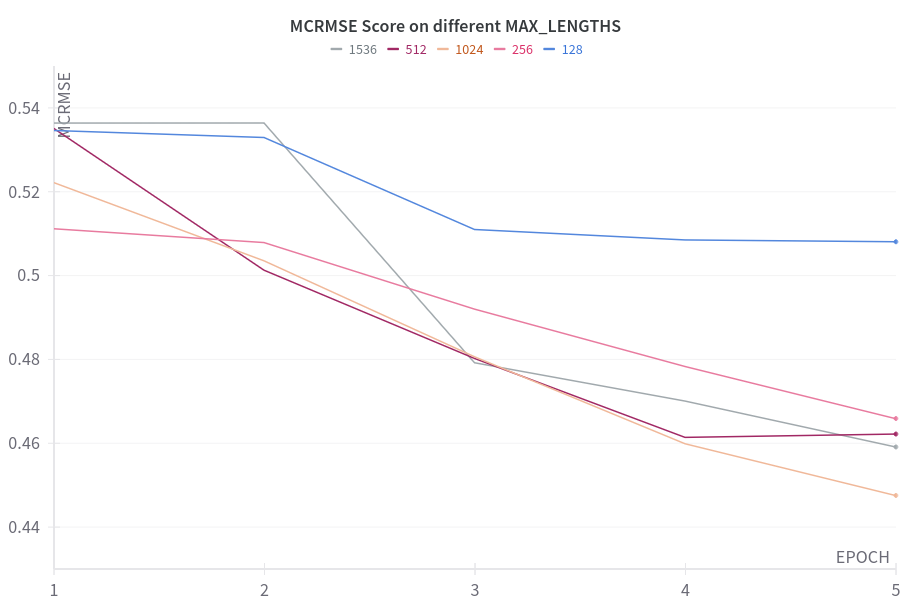
\includegraphics[keepaspectratio, width=0.9\textwidth]{img/max_length.png}
\caption{MCRMSE Score Evolution on different Max Lengths}
\label{fig:max_length}
\end{center}
\end{figure}

\subsubsection*{Hyperparameter configuration}
Below are the hyperparameters that were tuned and an explanation why the specific values were chosen.

\begin{itemize}
	\item \textbf{Max length:} 1024. Best performing max length.
	\item \textbf{Batch size:} 4. Maximum allowed batch size due to hardware limitation.
    \item \textbf{Epochs:} 4. MCRMSE Score converges at four epochs. Also, having too many epochs could lead to overfitting.
    \item \textbf{Learning rate:} 0.0001. Automatically fine-tuned using optuna\footnote{\href{https://optuna.org/}{Optuna - Automatic Hyperparameter Optimizer}}.
    \item \textbf{Weight decay:} 0.01. Automatically fine-tuned using optuna.
    \item \textbf{Hidden dropout prob:} 0.07. Automatically fine-tuned using optuna.
    \item \textbf{Attention probs dropout prob:} 0.07. Automatically fine-tuned using optuna.
\end{itemize}
\textbf{NOTE:} Hyperparameters which are not listed above use the default settings from the HuggingFace Library.


\subsubsection{Transformer result}
As seen in Figure~\ref{fig:deberta_performance}, the performance on the content score is high. However, improvements can be made on the wording score.

\begin{figure}[H]
    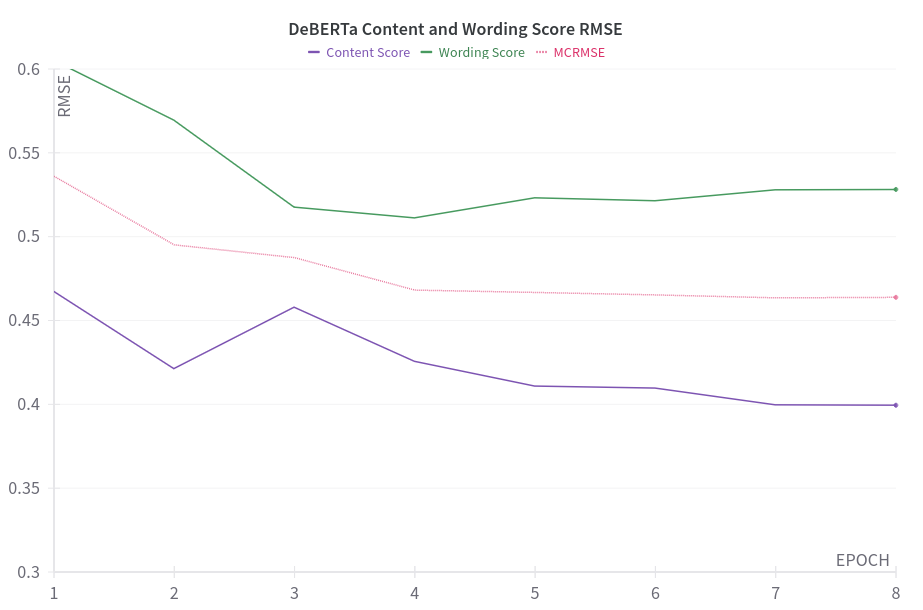
\includegraphics[keepaspectratio, width=\textwidth]{img/Deberta-performance.png}
\caption{Deberta Performance on Wording and Content}
\label{fig:deberta_performance}
\end{figure}

\pagebreak
\subsection{LightGBM}
\subsubsection{Motivation}
Being a GBDT-based model, LightGBM models are highly accurate without the need for powerful GPUs. Amongst contestants of this and various other Kaggle challenges, this machine learning algorithm is one of the most popular ones, often achieving the top rank on the Kaggle leaderboards of said challenges. Given that the prediction values, 'content' and 'wording', are continuous, numeric values it made sense to use a regression-based approach as well.
However, unlike other approaches used in this project, this approach requires more preprocessing and engineering of the data to get the best results.

\subsubsection{Preprocessing}
Like other traditional machine learning approaches, LightGBM does not directly work with text data. Thus features like the student summaries themselves, could not be used as an input. Instead, the creation of new numeric features containing different information about the summaries and the prompts was necessary. Many of the new features in the final dataset were created using a library called 'Textstat' \parencite{a2022_textstattextstat}.  %citation or footnote with link?: \footnote{\href{https://github.com/textstat/textstat}{Textstat - GitHub Webpage}}
The Textstat library calculates different statistics from text. It helps determine readability, complexity, and grade level of the given student summaries. \\ Additionally, the number of overlapping N-grams between a reference text and a student summary were calculated and a separate \gls{rouge}-score was calculated as well. The motivation in using Textstat came from a discussion of a previous CommonLit challenge called the "CommonLit Readability Prize".
%\footnote{\href{https://www.kaggle.com/c/commonlitreadabilityprize}{CommonLit Readability Prize - Website}}
The notebook on that discussion can be found under \cite{yhirakawa_2021_textstat}. By using this library, the wording score improved compared to the other models used in this project.

\subsubsection{Architecture}
The LightGBM model only uses the student summaries and the reference texts. New features are created from those two input features using Textstat, as described above. The data then gets split into three sets: 80\% for training, 10\% for validation and 10\% for testing. This choice was made due to this split being very common in the field of machine learning.  %Put this in the Data chapter?
The hyperparameters were tuned on the validation set using Optuna and finally everything was evaluated on the test set. The final output consisted of the wording and content scores of all the student summaries.
A graphical representation of this process can be found in Figure~\ref{fig:lightgbm-model}.

\begin{figure}[H]
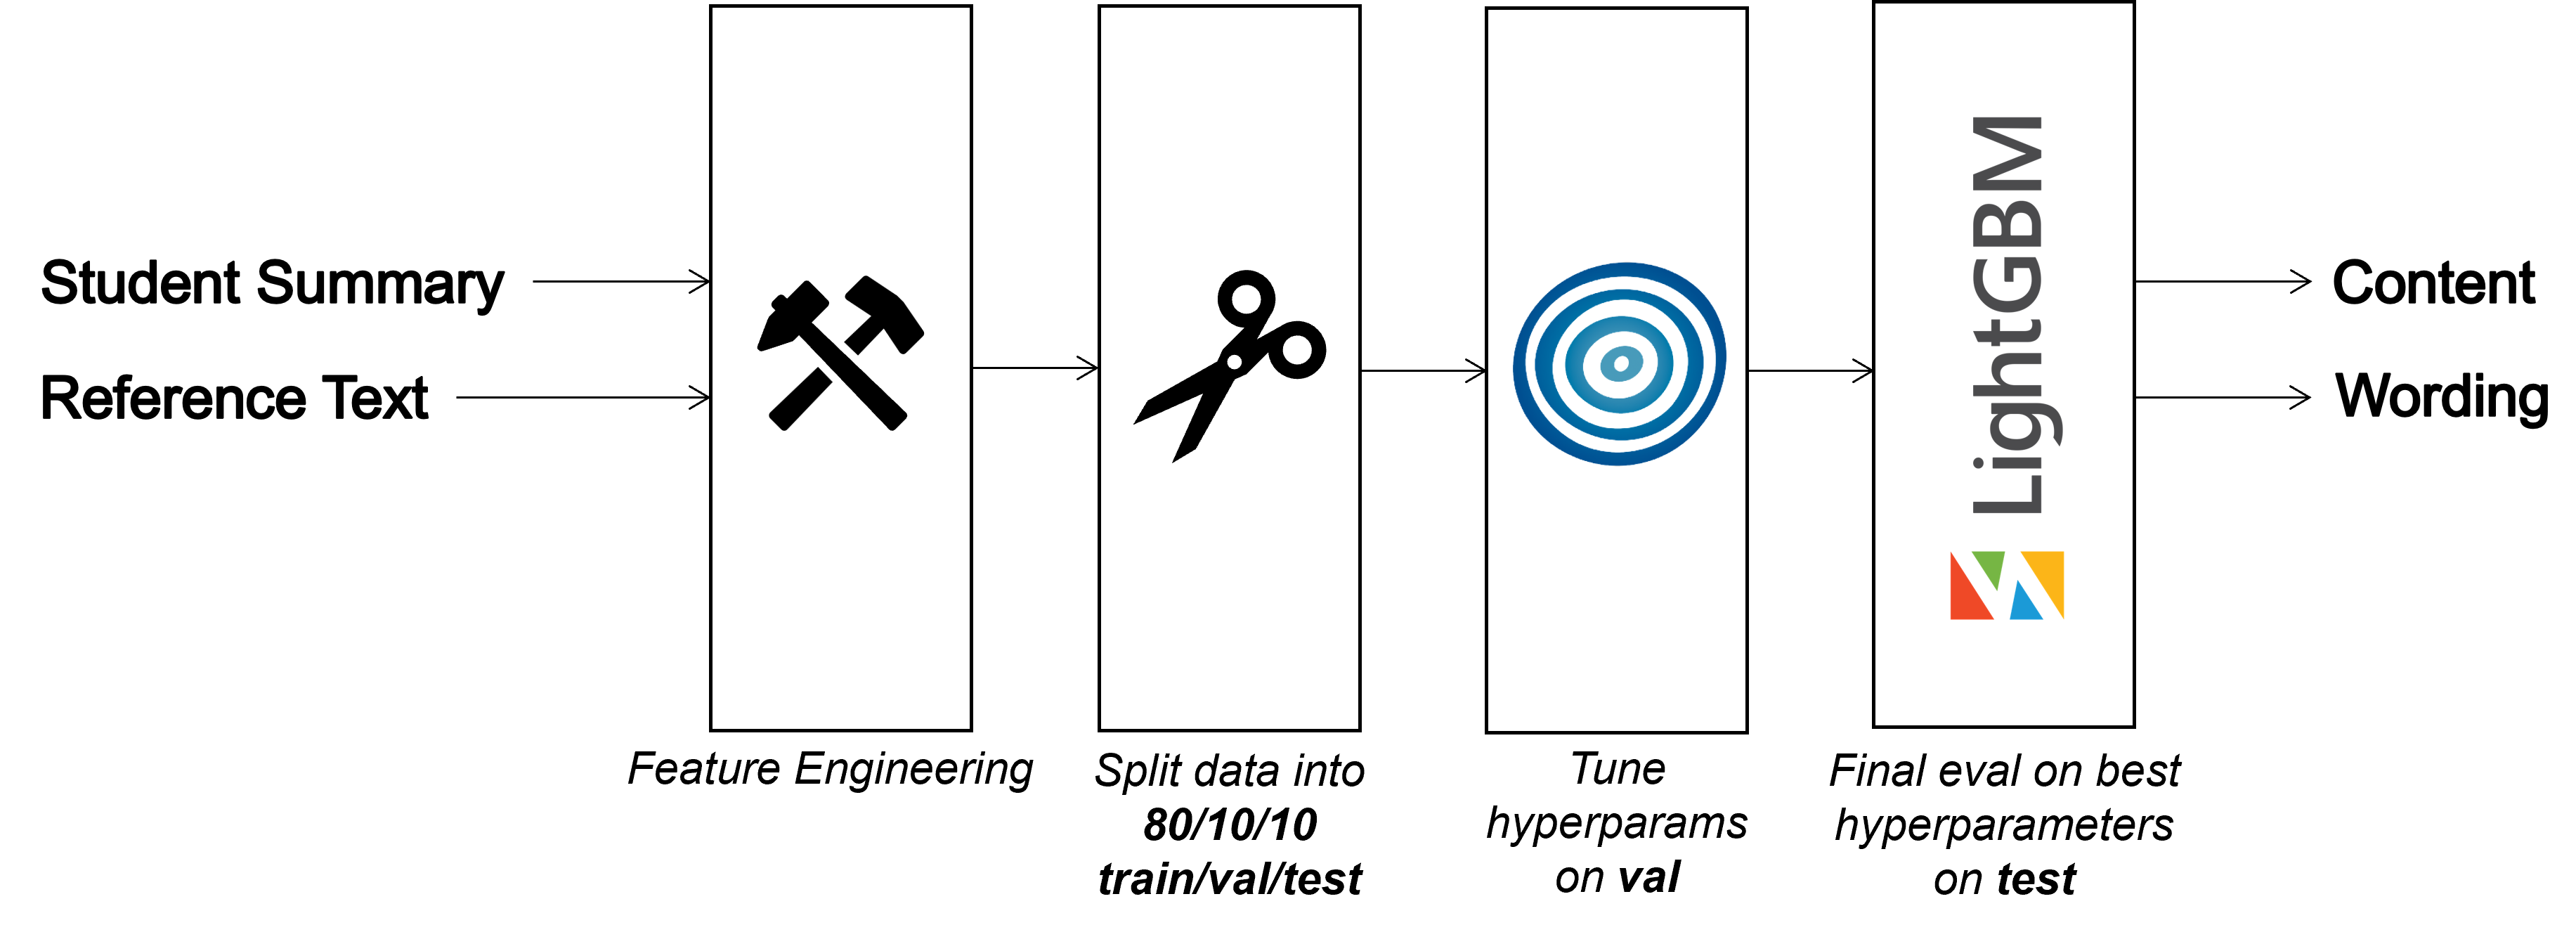
\includegraphics[keepaspectratio, width=\textwidth]{img/lightgbm-architecture.png}
\caption[Pipeline of the LightGBM Model]{Pipeline of the LightGBM model, the feature engineering was done using the aforementioned Textstat library and the hyperparameters were tuned with the help of Optuna}
\label{fig:lightgbm-model}
\end{figure}

\subsubsection{Hyperparameters}

For the LightGBM model, Optuna was used. Optuna allows for efficient hyperparameter tuning by optimizing an objective function. Additional details can be found by referring to the original article under \cite{10.1145/3292500.3330701}.\\

\noindent These are the final hyperparameters that have been used for this model:

\begin{itemize}
	\item \textbf{Number of Estimators
:} 778
	\item \textbf{Learning Rate
:} 0.015
	\item \textbf{Colsample Bytree
:} 0.761
	\item \textbf{Reg Alpha
:} 0.002
\end{itemize}

\noindent Those final hyperparameters have been used after using Optuna to determine the importance of every hyperparameter and only using those four, which had the highest importance. This was done to maximize the hyperparameter search speed for any subsequent training. Any definitions can be found in the glossary.

\subsubsection{Results}

The final \gls{mcrmse} scores of the LightGBM model were as follows:

\begin{itemize}
	\item \textbf{Content RMSE:} 0.66
	\item \textbf{Wording RMSE:} 0.51
	\item \textbf{MCRMSE:} 0.59
\end{itemize}

\noindent This model performs better on the wording score than the other approaches in this project. This was one of the reasons for choosing an ensemble-based approach to improve the final score.


\subsection{Ensemble}
The Ensemble Model merges the predictions from the three models above: the ROUGE-Based Model, the LightGBM Model and the Transformer, as shown in
\hyperref[fig:ensemble-model]{Figure~\ref{fig:ensemble-model}}.
Each of these models independently predicts both content and wording scores, which the Ensemble Model combines into the two final scores.

\subsubsection{Model Architecture}

The summary, reference text, and the prompt are provided as raw text inputs for this ensemble. Each of the three individual models perform their own preprocessing steps on the texts. (These steps are explained in their respective sections above).
Following preprocessing, the models make their predictions, which the ensemble aggregates using a single linear layer, down-projecting them into the two final predictions. The linear layer is trained to predict scores based on the outputs of the three models, effectively learning how to weigh each model's contribution. Instead of a simple (weighted) average, the ensemble learns to leverage the strengths of each model: the ROUGE-Based Model performs well on the content score, LGBM on the wording score, and the Transformer is a great generalizer that also takes the specific question of the task into consideration.

\begin{figure}[H]
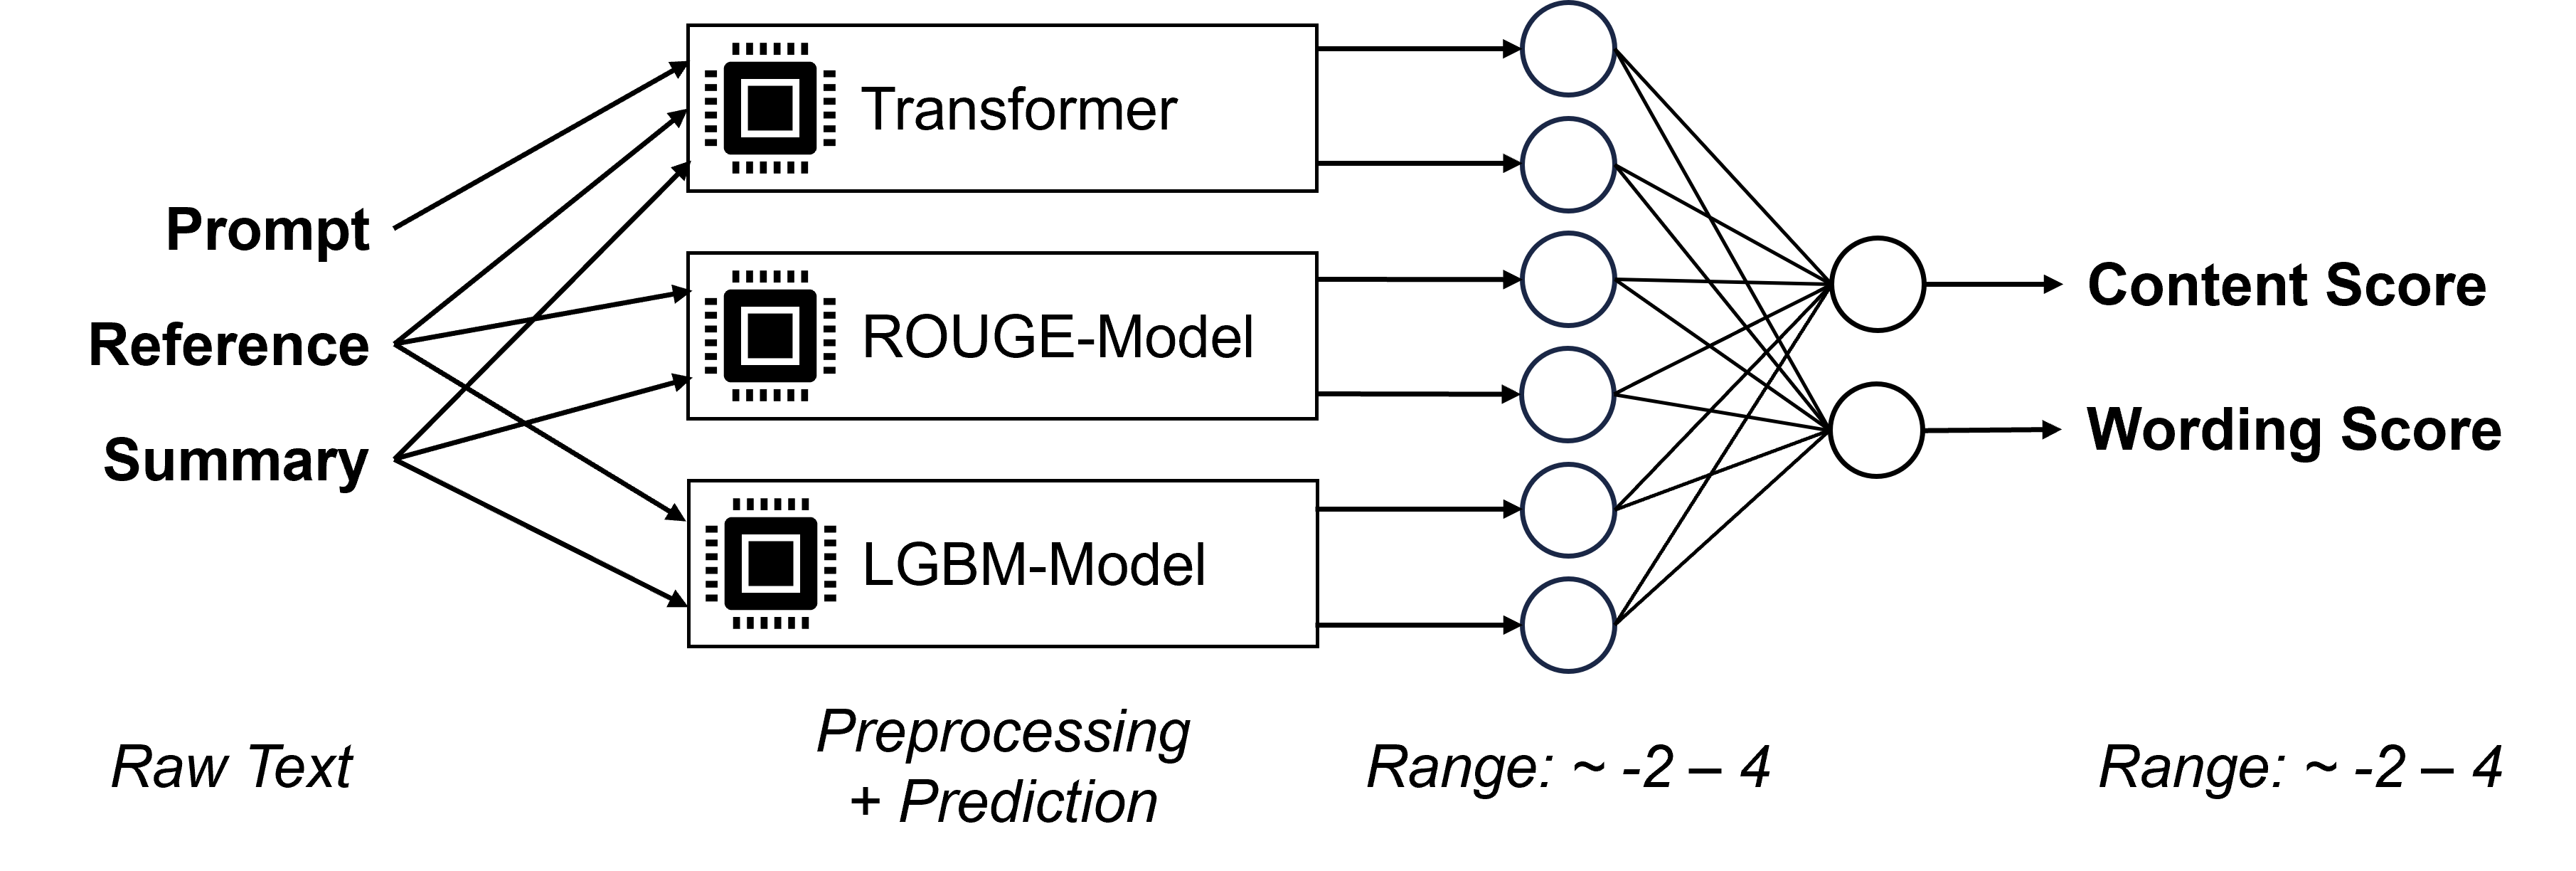
\includegraphics[keepaspectratio, width=\textwidth]{Ensemble-Model.png}
\caption{Architecture of the Ensemble-Model.}
\label{fig:ensemble-model}
\end{figure}

\subsubsection{Hyperparameter Tuning}

The "learned weighted average" approach was the only one investigated for this model. Since the model consists of just one linear layer, there were only a few parameters to test. While experimenting with hidden layers for this model, it became clear quite quickly that the added non-linearity, no matter the \gls{activation function}, reduced performance. However, like the ROUGE-Based Model, the simplicity meant that the Ensemble Model was robust against overfitting as well as changes to the \gls{lr} and the number of training \glspl{epoch}. Leading to the following hyperparameters:

\begin{itemize}
    \item \textbf{\glsdisp{hidden-layer}{Hidden-Layers}:} 0 Hidden Layers
    \item \textbf{\glsdisp{hidden-dim}{Hidden-Dim}:} 0 Neurons 
    \item \textbf{\glsdisp{activation function}{Activation Function}:} No Activation Function
    \item \textbf{\glsdisp{lr}{Learning Rate}:} 0.01
    \item \textbf{\glsdisp{epoch}{Epochs}:} 10 Epochs
\end{itemize}


\section{Model Evaluation}
\subsection{Results}
The performances of the developed models were assessed using the \gls{mcrmse}. The final Kaggle scores, representing the Ensemble Models' performance and generalization capabilities, are as follows:

\begin{itemize}
    \item \textbf{Final Public Score:} 0.4956
    \item \textbf{Final Private Score:} 0.4977
\end{itemize}
% \begin{figure}[h]
% 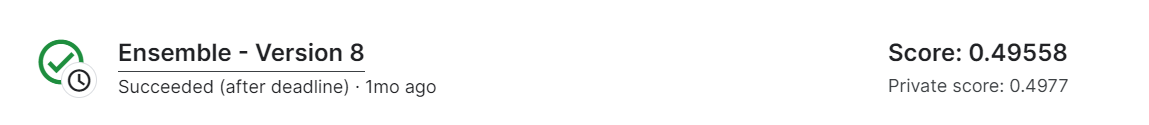
\includegraphics[keepaspectratio, width=\textwidth]{final_score_kaggle.png}
% \caption{Final Kaggle Score}
% \label{fig:rouge-correlation-matrix}
% \end{figure}
Furthermore, the Ensemble Model was evaluated on a separate test set, with scores during training and testing phases:

\begin{itemize}
    \item \textbf{Final Training-Set Score:} 0.3687
    \item \textbf{Final Test-Set Score:} 0.4981
\end{itemize}

\subsubsection{Evolution of Kaggle Scores}

The following graphs
(\hyperref[fig:kaggle-score-evolution]{Figure~\ref{fig:kaggle-score-evolution}}
and
\hyperref[fig:kaggle-score-evolution_clipped]{Figure~\ref{fig:kaggle-score-evolution_clipped}})
illustrate the evolution of Kaggle scores throughout the development process. Some models, like the RNN and LSTM are not listed as they were not tested thoroughly, and those with multiple entries have some variation in their hyperparameters. The full range and a clipped version of the graph - highlighting the lowest (best) scores - show the progress of the models and their performances.

\begin{figure}[H]
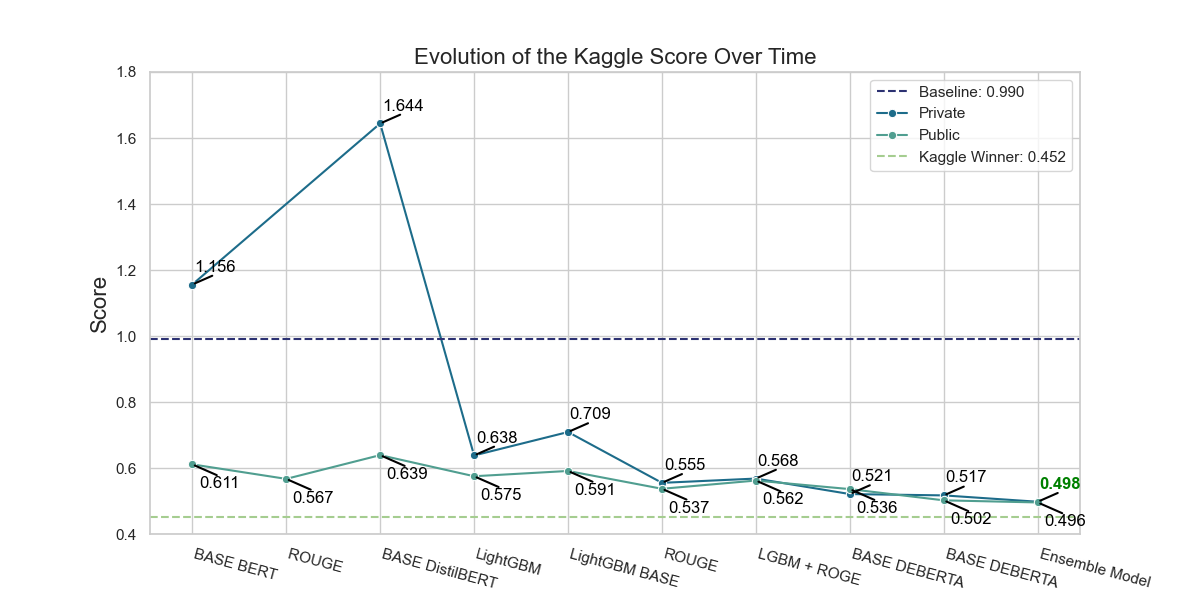
\includegraphics[keepaspectratio, width=\textwidth]{Kaggle_Score_Evolution_(Full).png}
\caption{Kaggle Score Evolution}
\label{fig:kaggle-score-evolution}
\end{figure}
\begin{figure}[H]
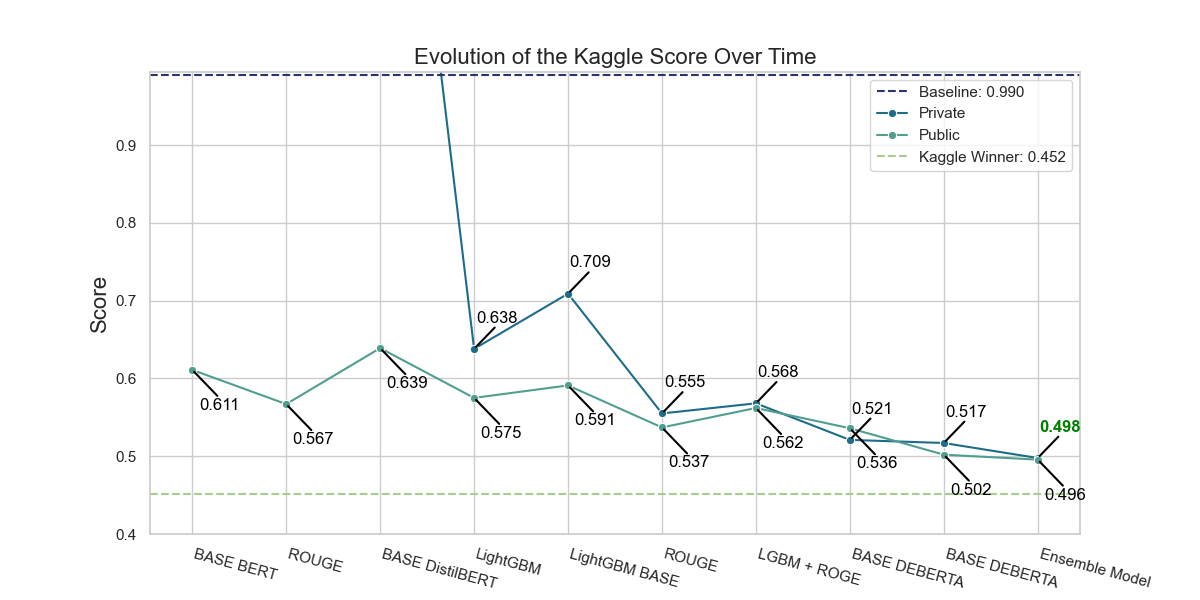
\includegraphics[keepaspectratio, width=\textwidth]{Kaggle_Score_Evolution_(Clipped_1).png}
\caption{Kaggle Score Evolution (Clipped at the Baseline score)}
\label{fig:kaggle-score-evolution_clipped}
\end{figure}


\pagebreak
\subsection{Error Analysis}
The final evaluation of the project involved assessing the performance of the ensemble model on the test set, which was 20\% of the provided data. The final score was 0.498, consistent with the scores achieved in the Kaggle competition, suggesting a representative outcome.

\subsubsection*{Error distribution}
\begin{figure}[H]
    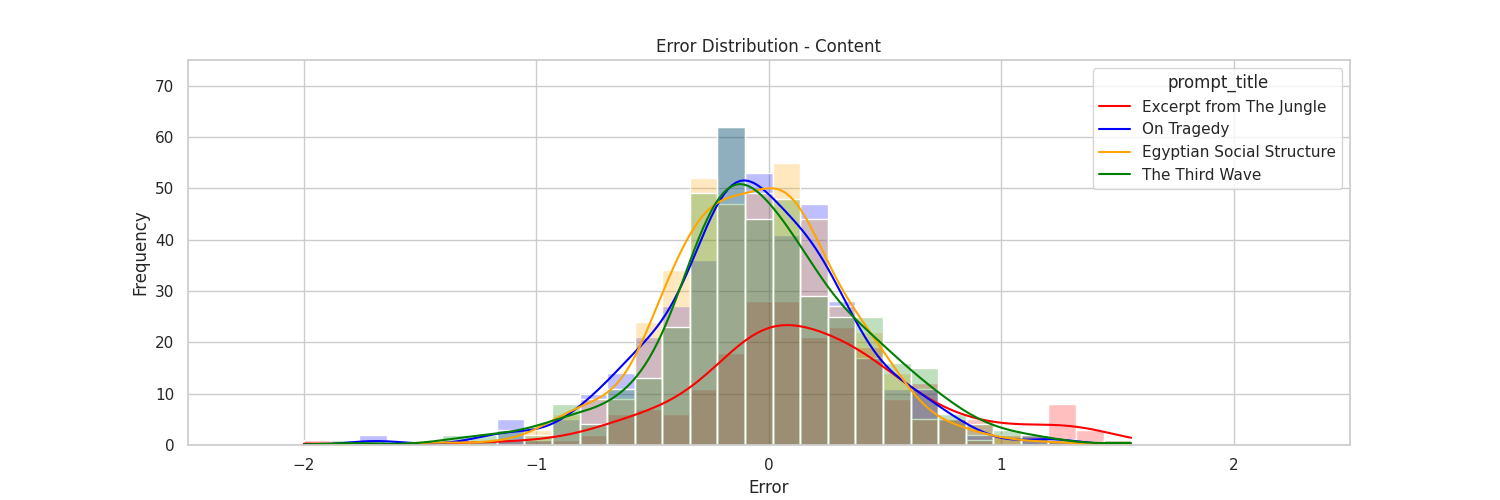
\includegraphics[keepaspectratio, width=\textwidth]{error_distribution_content.png}
    \caption{Error Distribution - Content}
    \label{fig:error_distribution_content}
\end{figure}
\begin{figure}[H]
    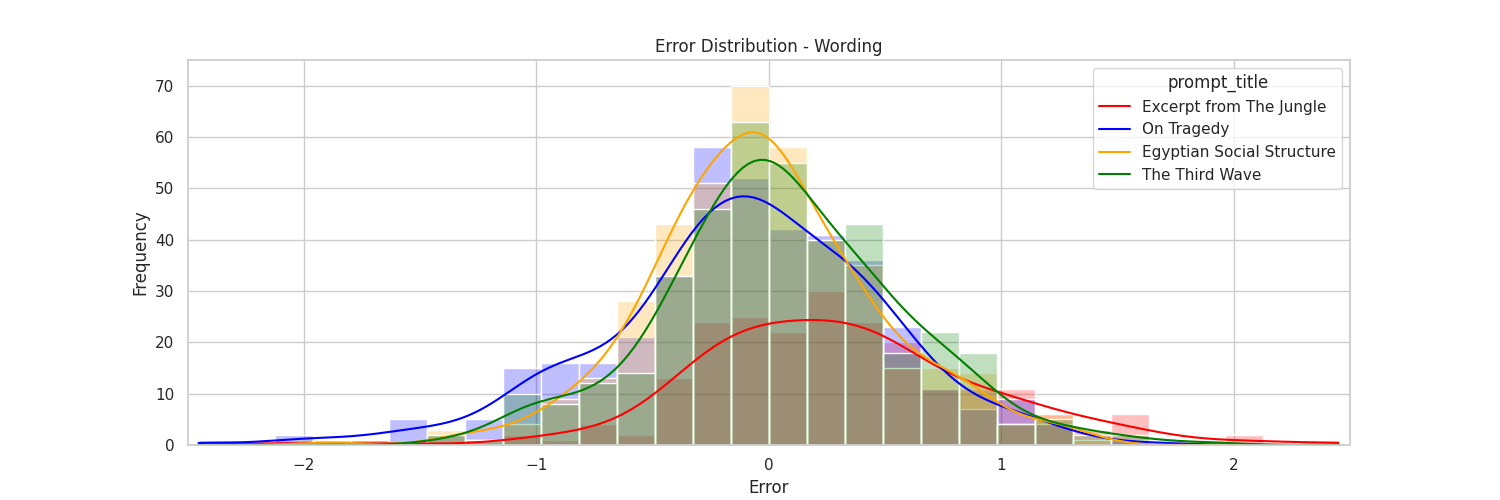
\includegraphics[keepaspectratio, width=\textwidth]{error_distribution_wording.png}
    \caption{Error Distribution - Wording}
    \label{fig:error_distribution_wording}
\end{figure}
The analysis of the error distribution for content and wording scores, as illustrated in Figures \ref{fig:error_distribution_content} and \ref{fig:error_distribution_wording}, 
reveals a gaussian distribution peak around zero, with most errors being smaller than 1. This suggests that the model's errors are generally small in magnitude. The even distribution also shows that the model does not tend to predict to high nor too low.

\subsubsection*{Mean absolute error}

\begin{figure}[H]
    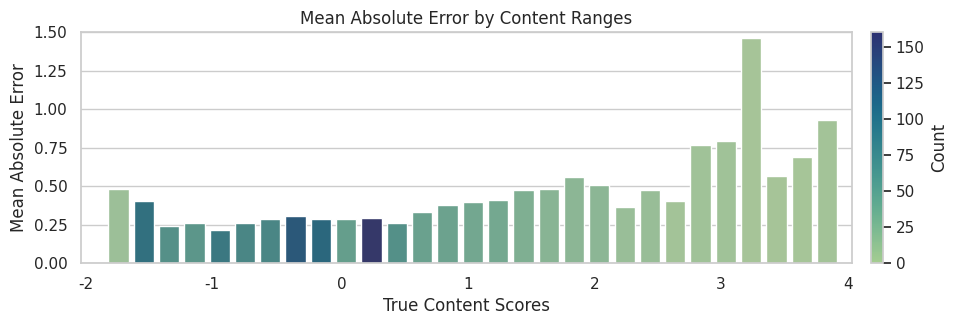
\includegraphics[keepaspectratio, width=\textwidth]{mean_absolute_error_content.png}
    \caption{Mean Absolute Error - Content}
    \label{fig:mean_absolute_error_content}
\end{figure}
\begin{figure}[H]
    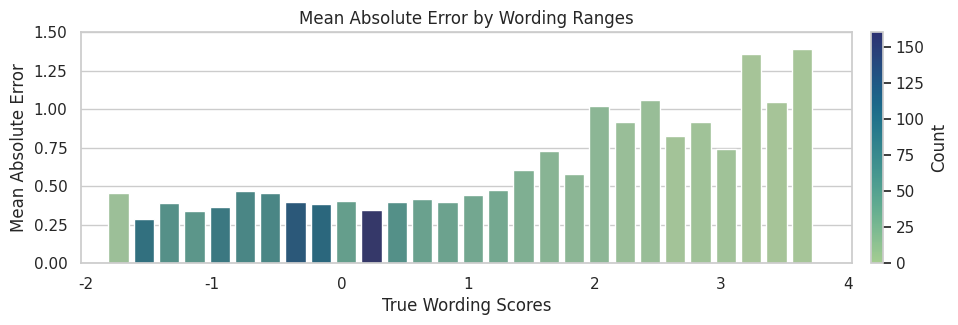
\includegraphics[keepaspectratio, width=\textwidth]{mean_absolute_error_wording.png}
    \caption{Mean Absolute Error - Wording}
    \label{fig:mean_absolute_error_wording}
\end{figure}
Displayed above are plots illustrating the \gls{mae} for the true content and wording scores. (Figure~\ref{fig:mean_absolute_error_content} and Figure~\ref{fig:mean_absolute_error_wording}) These plots use color intensity to represent data density: lighter shades indicate less training data in the dataset.
These plots reveal a tendency for higher \glspl{mae} in areas with lighter colors, suggesting that the model has difficulties with less frequent data. It can be inferred that an increase in data quantity within these lighter ranges would likely enhance the models performance.


\section{Discarded Approaches}

\subsection{RNN \& LSTM}
%\subsubsection*{Motivation}
Since \glspl{rnn} and \glspl{lstm} are specifically designed for processing sequential data, making them particularly effective for handling text and tasks involving natural language, they served as ideal starting points for early prototyping.\\

\glspl{rnn} and \glspl{lstm} formed the initial approach, primarily exploring the wording metric, in the hopes that these models could assess the use of objective language and evaluate the use of lexis and syntax. This approach also allowed the team to get comfortable with the dataset, preprocessing techniques, as well as model implementation and training with PyTorch\footnote{\href{https://pytorch.org/}{PyTorch - Website}}, tracking with Weights \& Biases (WandB)\footnote{\href{https://wandb.ai/site}{Weights \& Biases - Website}} and a models evaluation processes. However, this first approach was discarded in favor of other models that had better performance for comparable efforts.

\subsubsection{Model Architectures}
Both the \gls{rnn} and \gls{lstm} models used a similar bidirectional architecture featuring a linear classifier as output. Stopwords were removed from the summaries, the remaining words were uncapitalized and stemmed to their base forms. Each of these \glsdisp{token}{word-tokens} were vectorized using \gls{w2v}. These encoded strings then got passed into the model sequentially. After processing each \gls{token}, the classifier generated the prediction for the wording score of that summary.\\ 

\subsubsection{Hyperparameters}
\begin{itemize}
    \item \textbf{Model Type:} Whether the Model is an RNN or an LSTM.
	\item \textbf{Embedding-dim.:} Dimensionality of the word embeddings.
	\item \textbf{Hidden-dim.:} Dimensionality of the hidden layers.
	\item \textbf{Num Layers:} Number of layers in the RNN or LSTM.
	\item \textbf{Epochs:} Number of training Epochs.
\end{itemize}

%\subsubsection{Training}
%The training of both \gls{rnn} and \gls{lstm} models involved optimizing the models’ parameters using the Adam optimizer. The \gls{mse} loss function was utilized, measuring the difference between the predicted wording scores and the actual scores. The models were trained for twenty epochs, and the training process was monitored using the WandB platform for experiment tracking.

\subsubsection{Limitations}
These models struggled with overfitting. Notably, \glspl{rnn} achieved a suspiciously impressive \gls{rmse} score of 0.03 for wording on the training set. This success did not generalize well to the validation set, where \gls{rmse} scores got as high as 2.25, well above the baseline of 0.99. The complex nature of the natural language in the summaries posed challenges for these models. Also, considering that the models only looked at the summaries themself, without comparing them to the reference texts, it was decided to no longer pursue this approach.


\subsection{DeBERTa Large}
After having success with the DeBERTa Base model, there was hope that using the DeBERTa Large model would lead to a better performance.
However, after experimenting with the large model there was an overfitting problem.
The initial intention was to allocate more time to solving this problem. However, the extensive number of parameters resulted in longer training times. 
Additionally, hardware limitations and time constraints necessitated the decision to discard this approach. Potentially, with extended time and enhanced computing power, better performance could be achieved.

% Modeling
% Models - All
% 	LSTM - Josef
% 	ROUGE - Josef
% 	Transfromer - Jonathan
% 	LGBM - Tarrmeehan
% 	Ensemble - Josef
% Model Evaluation - Josef
% Error Analysis and Improvements - Jonathan

\chapter{Conclusion}
% End-Ergebnisse und kritische Wertung
Overall, the team is satisfied with the project result. This was the first Kaggle challenge for all four members.
The team was able to place 975th out of a total 2065 participants, with a private score of 0.4977 on the already finished Kaggle competition leaderboard:
\vspace{1em}


\begin{figure}[H]
    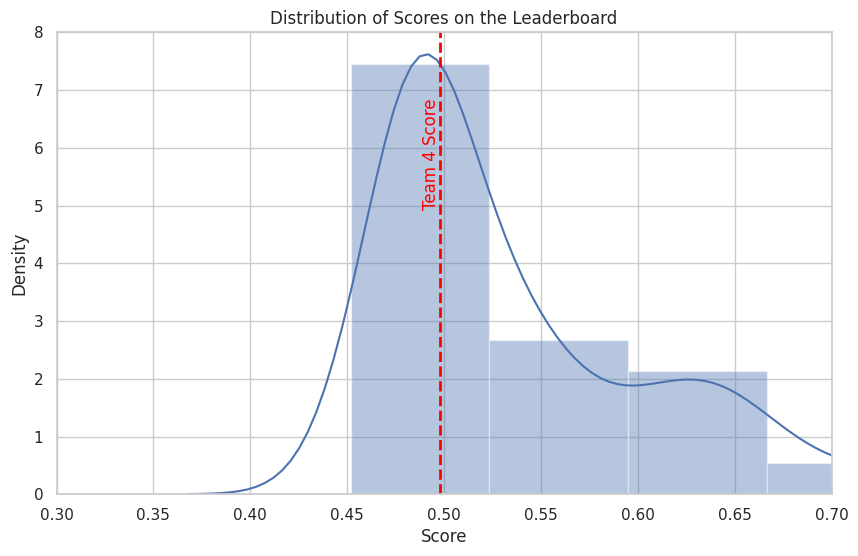
\includegraphics[keepaspectratio, width=\textwidth]{score_dist.png}
\caption{Kaggle Score Distribution}
\label{fig:score_dist}
\end{figure}
\vspace{1em}

\noindent When looking at the winning solution, it became apparent that developing a similar approach would be challenging due to the complexity and depth of the winner's strategy.
In summary, the leader used Large Language Models with specific prompts to augment data, coupled with a four-fold transformer ensemble.
\\

\noindent With the absence of time constraints and hardware limitations, the team could have explored additional approaches. This might have involved using a larger DeBERTa model or dedicating more time to the development of the ensemble. Nevertheless, the achieved results are considered satisfactory, given the unique solution employed.
The solution combines a deep-learning approach such as transformers and a linguistic approach 
such as \gls{rouge}-Based Model and LightGBM with linguistic features.

 





\section{Challenges and Lessons Learned}
At the beginning of the project, none of the team members had completed the Natural Language Processing course.
Instead, the NLP course was taken in parallel with the AI Challenge course.
This made it especially difficult to work with transformers, since they are quite an large topic to understand.
While on the topic on transformers, they are computationally intensive models and,
even with the provided hardware from the university, computing limitations were still an issue.
This was not the only challenge; the team also never worked with or implemented an ensemble.
Nevertheless, with these challenges the team has definitely learned a lot in the field of NLP and how machine learning in general can be used in real life settings.


\chapter{Reflection}
At the beginning of the challenge there was not a lot of motivation coming into the project.
When selecting the competition, we did not find a topic that seemed interesting to us and just settled for "Evaluate Student Summaries".
But as time went by, we grew to enjoy the challenge, especially after implementing our own ideas to solve the problem.
Communication within the team and with our coach was a strong point. We consistently received valuable feedback and could freely discuss machine learning queries. 
Our approach to planning was systematic, with weekly goals and milestones that kept us on track. Notably, our presentation skills noticeably imporved with each successive presentation.

\vspace{1em}

\noindent At the end of the day, we feel that the AI Challenge course served as a good preparation for the upcoming Bachelor Thesis
and are thankful for the opportunity as we are now more confident to write and present any technical project.
% Fazit zur Challenge & Lessons learned

% Conclusion - Jonathan
% Reflection - Jonathan

\newpage

\pagenumbering{Roman}

\appendix
% Verhindert das Einfügen von Kapiteltitel kleiner als \chapter
\addtocontents{toc}{\protect\setcounter{tocdepth}{0}}

\printglossaries

\listoffigures

\listofmyequations \pagebreak

\printbibliography

version https://git-lfs.github.com/spec/v1
oid sha256:a8b9f337b508410b8f5beeda2282fee50f157c3e4b0032aaf22fd91d2d6a234d
size 108


\end{document}
